% Drop-in replacement for Sections "A Precision Farming Scenario" and "Experiments" of 9_GEGF.tex.
% Needs: \usepackage{booktabs}; tables/figures are produced by run_all.py (folder results/).
% Listing labels follow the draft: freshness, sensitivity, frequencyprotocol, criticalityprotocol,
% listing1, listing2, listing3new, listing4, recipient.

\section{A Precision Farming Scenario}\label{sec:scenario}
Consider a smart greenhouse cultivating high-value tomatoes. The \textsf{data layer} ($d_n$) holds soil-moisture,
temperature, humidity, and nutrient sensors, canopy cameras, scouting drones, and agricultural records (cultivation,
irrigation, fertilization, and historical/external datasets). The \textsf{edge layer} ($e_n$) holds greenhouse
gateways ($e_{n1}$--$e_{n3}$) running irrigation control and computer vision. The \textsf{cloud layer} ($c_n$) holds
cloud nodes ($c_{n1}$, $c_{n2}$) for analytics, archiving, and model training.

\paragraph{Labels.} Each data item and each job carries labels that the policies evaluate. \textit{Static} labels are
set by the owner; \textit{dynamic} labels are computed at run time (Table~\ref{tab:labels}).

\begin{table}[htbp]\scriptsize\centering
\caption{Labels used in the scenario (policy references use \texttt{\textbackslash ref}, not hard-coded numbers).}\label{tab:labels}
\begin{tabular}{llllll}
\toprule
Item & Label & Value & Type & Assigned by & Policy\\
\midrule
Reading / frame & Freshness \& value (utility) & $H(d)\ge\theta$ & dynamic & sending node & Listing~\ref{freshness}\\
 & Frequency & continuous / intermittent & dynamic & sender per segment & Listing~\ref{frequencyprotocol}\\
 & Sensitivity & high & static & farm operator & Listing~\ref{sensitivity}\\
 & Value (risk) & high (readings) / low (frames) & static & farm operator & Listing~\ref{criticalityprotocol}\\
Irrigation job & Criticality / Confidentiality & high / low & static & job owner & Listing~\ref{recipient}\\
Disease-detection job & Criticality / Confidentiality & low / high & static & job owner & Listing~\ref{recipient}\\
Fertigation-planning job & Criticality / Confidentiality & high / high & static & job owner & Listing~\ref{recipient}\\
Archiving job & Criticality / Confidentiality & low / low & static & job owner & Listing~\ref{recipient}\\
\bottomrule
\end{tabular}
\end{table}

\paragraph{$\mathcal{DF}_1$ (data $\rightarrow$ edge $\rightarrow$ cloud): irrigation control.}
Soil-moisture and soil-temperature readings must reach the greenhouse gateway while still fresh; only the processed
result (irrigation events, 15-minute zone summaries) goes to the cloud. \textit{Data:} a reading enters the flow
only if $H(d)\ge\theta$ (Listing~\ref{freshness}); static metadata and repeated overnight readings fall below $\theta$
and stay at the sensor. \textit{Protocol:} readings are sensitive (they reveal growing practices) and high-risk
(a lost reading may cause a missed irrigation cycle), so Listings~\ref{frequencyprotocol}, \ref{sensitivity}, and
\ref{criticalityprotocol} apply together. On the data-to-edge segment the stream is continuous, and MQTTS with QoS~1
is the only protocol satisfying all three (encrypted, persistent session, delivery confirmed). On the edge-to-cloud
segment the derived items are intermittent but remain sensitive and high-risk, so HTTPS applies. \textit{Job:} the
irrigation job is critical and non-confidential; candidates are narrowed to the greenhouse edge nodes, and
Listing~\ref{recipient} prohibits any node with $A(n)<\alpha$. If $e_{n1}$ is overloaded or down, the job is offloaded
to a peer edge node and, failing that, to a cloud node, provided the freshness deadline still holds.

\paragraph{$\mathcal{DF}_2$ (data $\rightarrow$ edge$|$cloud): disease evidence.}
Canopy frames showing early disease symptoms are valuable and sensitive: the edge needs them now to trigger
treatment, and the cloud needs the raw copy for audit and model re-training. Listings~\ref{listing3new} and
\ref{listing4} state that both recipients receive the data concurrently, over a lightweight protocol (MQTTS) to the
edge and a bandwidth-capable one (HTTPS) to the cloud. Disease detection is confidential but not critical, so it may
run only on nodes with $T(n)\ge\tau$ (e.g., $e_{n1}$, $e_{n2}$, $c_{n1}$, not $e_{n3}$ or $c_{n2}$).

\paragraph{$\mathcal{DF}_3$ (data $\rightarrow$ edge): proprietary fertigation recipes.}
Fertigation set-points and nutrient telemetry must not leave the greenhouse. Listing~\ref{listing1} is reused as-is
and no obligation analogous to Listing~\ref{listing2} exists. The fertigation-planning job is both critical and
confidential, so it needs a node that is available \emph{and} trusted; if none qualifies, the fallback of
Listing~\ref{recipient}'s discussion applies (initiator, priority queue, or rejection).

\paragraph{$\mathcal{DF}_4$ (data $\rightarrow$ cloud): historical and external datasets.}
Multi-season crop records, weather, satellite, and market data are bulky and not time-critical. They bypass the edge
and go directly to the cloud, where abundant resources train the yield and disease models. The archiving and training
jobs are non-critical and non-confidential, so any cloud node may receive them.

\paragraph{$\mathcal{DF}_5$ (data $\rightarrow$ cloud $\rightarrow$ edge): model updates.}
Cloud-trained models and weekly yield forecasts flow back to the greenhouse. Data criticality prevails over freshness.
The policies for $\mathcal{DF}_4$ and $\mathcal{DF}_5$ are not yet developed in the paper; the scenario is stated here,
but they are \emph{not} evaluated below.

\section{Experiments}\label{sec:experiments}

\subsection{Setup}
We evaluate the policies on a purpose-built, seeded discrete simulator of the scenario (\texttt{experiments/farm/}).
Section~
ef{sec:ifogsim} repeats the experiments on iFogSim2. The first simulator is purpose-built: the policy documents themselves (Listings~\ref{freshness} and~\ref{recipient}, as JSON) are
evaluated by a small ODRL evaluator (permission, prohibition, \texttt{conflict=prohibit}), so each decision comes from
the listing and not from hand-coded logic. All parameters below are assumptions, not measurements.

\paragraph{Data-flow workload (E1).} A 6-hour window (03:00--09:00, sunrise at 06:00), 40 soil sensors (60\,B every
30\,s), 12 cameras (150\,kB every 5\,s). Each item is \emph{useful} (it informs irrigation/vision) with probability
0.10--0.70 rising at sunrise; entropy $H(d)$ is a noisy proxy (useful: Beta(5,2); other: Beta(1.5,8)). Three
gateways have two inference slots each (frame service time 1.8\,s) and drop items that wait over 20\,s. The farm
uplink is 2\,Mbit/s, shared by all cloud-bound traffic and modelled as a fluid queue (delay $\propto 1/(1-\rho)$,
tail drop beyond 95\,\% load). Wireless link loss is 2\,\%. Freshness deadlines: 2\,s (readings), 8\,s (frames).

\paragraph{Job workload (E2, E3).} Poisson arrivals over 30\,min of four job types (Table~\ref{tab:labels}; mix
45/25/10/20\,\%; deadlines 2/15/10/120\,s). Three edge nodes (2 slots, $T$=0.90/0.85/0.55) and two cloud nodes
(8 slots, 4$\times$ faster, $T$=0.95/0.50, 50/70\,ms away, behind the shared uplink). Edge nodes fail with MTBF 20\,min
and MTTR 1\,min. $A(n)=\max(0,1-\text{jobs in system}/\text{slots})$, and $0$ while down. \emph{Edge load} is the
offered edge work divided by edge capacity. Defaults: $\theta=0.3$, $\alpha=0.25$, $\tau=0.7$.

\paragraph{Baselines.} \textbf{E1:} \textsf{UG} (ungoverned: everything is forwarded over plain MQTT, QoS~0),
\textsf{SS} (static-secure: everything over HTTPS). \textbf{E2:} \textsf{random}, \textsf{cloud-only},
\textsf{static} (home edge; archiving in the cloud), and \textsf{greedy} (earliest estimated completion over all
nodes, ignoring trust and availability criteria). \textsf{CEGF} narrows candidates to the flow's layer, applies
Listing~\ref{recipient}, and picks the earliest estimated completion among eligible nodes (that choice is
\emph{management}; the policy only decides eligibility). It offloads to peers/clouds when the preferred layer would
miss the deadline, and falls back to the initiator (critical) or holds and retries (confidential).

\paragraph{Metrics.} \textsf{Timely-useful} is the share of useful items whose result is available within the
deadline (counts filtered, lost, and dropped items as failures). Other metrics are uplink volume, edge wait, loss in
transit, sensor energy, share of unencrypted transfers, deadline misses, and policy violations (every placement is
audited against the policy in force when it was made). All results are means over 20 seeds with 95\,\% CIs.

\subsection{E1: governing data flows}
\paragraph{E1a -- governed vs.\ ungoverned $\mathcal{DF}_1$.}
\begin{table}[htbp]\scriptsize\centering
\caption{E1a -- DF$_1$ under three configurations (mean $\pm$ 95\% CI, 20 seeds); x1.5 = 50\% more cameras.}\label{tab:e1-df1}
\begin{tabular}{lrrrrrrr}
\toprule
Config. & Timely-useful (\%) & Uplink (MB) & Edge wait (s) & Stale drops & Useful-read.\ loss (\%) & Sensor energy (J/h) & Unenc.\ (\%) \\
\midrule
UG (x1.0) & 97.2\,$\pm$\,0.2 & 107\,$\pm$\,0 & 0.27\,$\pm$\,0.03 & 0\,$\pm$\,0 & 2.0\,$\pm$\,0.1 & 0.02\,$\pm$\,0.00 & 100\,$\pm$\,0 \\
SS (x1.0) & 99.2\,$\pm$\,0.3 & 164\,$\pm$\,0 & 0.28\,$\pm$\,0.03 & 0\,$\pm$\,0 & 0.0\,$\pm$\,0.0 & 1.38\,$\pm$\,0.00 & 0\,$\pm$\,0 \\
CEGF (x1.0) & 98.7\,$\pm$\,0.1 & 71\,$\pm$\,0 & 0.09\,$\pm$\,0.01 & 0\,$\pm$\,0 & 0.0\,$\pm$\,0.0 & 0.01\,$\pm$\,0.00 & 0\,$\pm$\,0 \\
UG (x1.5) & 0.1\,$\pm$\,0.0 & 148\,$\pm$\,0 & 18.24\,$\pm$\,0.05 & 8355\,$\pm$\,285 & 2.0\,$\pm$\,0.1 & 0.02\,$\pm$\,0.00 & 100\,$\pm$\,0 \\
SS (x1.5) & 0.1\,$\pm$\,0.0 & 213\,$\pm$\,0 & 18.57\,$\pm$\,0.05 & 11154\,$\pm$\,367 & 0.0\,$\pm$\,0.0 & 1.38\,$\pm$\,0.00 & 0\,$\pm$\,0 \\
CEGF (x1.5) & 97.5\,$\pm$\,0.2 & 101\,$\pm$\,0 & 0.32\,$\pm$\,0.02 & 0\,$\pm$\,0 & 0.0\,$\pm$\,0.0 & 0.01\,$\pm$\,0.00 & 0\,$\pm$\,0 \\
\bottomrule
\end{tabular}
\end{table}
At the nominal load CEGF forwards 44\,\% of the items, which cuts uplink traffic by 34\,\% (vs.\ UG) and 57\,\%
(vs.\ SS) and edge waiting by about 3$\times$. It loses no useful readings in transit, while UG loses 2\,\% (QoS~0) and
sends 100\,\% of sensitive data unencrypted. SS is compliant but costs about 100$\times$ more sensor energy (TLS
sessions). SS reaches a slightly \emph{higher} timely-useful ratio (99.2\,\% vs.\ 98.7\,\%): the entropy filter misses
1.1\,\% of useful items, which is the price of the volume reduction. With 50\,\% more cameras the edge is
overloaded (utilization $\approx$1.08) and UG and SS collapse (about 0\,\% timely, 8\,000--11\,000 stale drops),
whereas CEGF stays at 97.5\,\%.

\begin{figure}[htbp]\centering
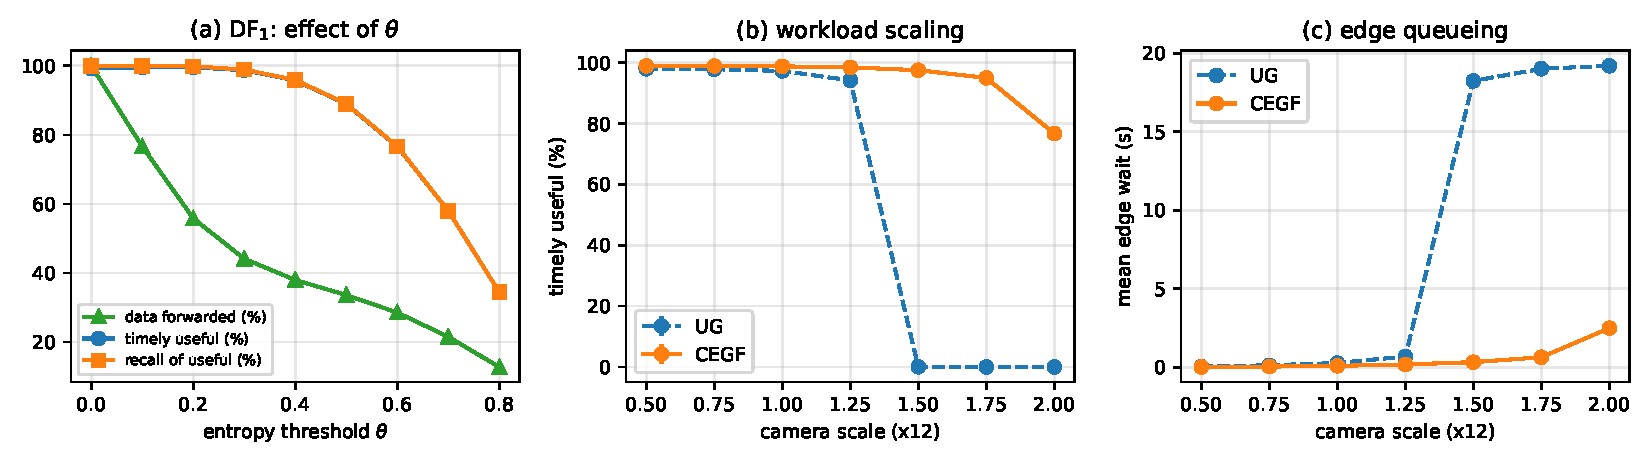
\includegraphics[width=\textwidth]{results/fig_e1.pdf}
\caption{E1: (a) entropy threshold $\theta$ in $\mathcal{DF}_1$; (b,c) timely-useful ratio and edge waiting vs.\
workload (camera scale; 1 = 12 cameras).}\label{fig:e1}
\end{figure}

\paragraph{E1b -- the four developed flows.}
\begin{table}[htbp]\scriptsize\centering
\caption{E1b -- the four developed data flows under CEGF policies (mean $\pm$ 95\% CI, 20 seeds).}\label{tab:e1-flows}
\begin{tabular}{lrrrrr}
\toprule
Flow & Timely-useful (\%) & p95 time-to-action (s) & p95 cloud delay (s) & Uplink (MB) & Sensor energy (J/h) \\
\midrule
DF$_1$ & 98.7\,$\pm$\,0.1 & 2.8\,$\pm$\,0.0 & 2.9\,$\pm$\,0.0 & 71\,$\pm$\,0 & 0.01\,$\pm$\,0.00 \\
DF$_2$ & 98.7\,$\pm$\,0.1 & 2.8\,$\pm$\,0.0 & 17.8\,$\pm$\,0.2 & 3420\,$\pm$\,7 & 0.65\,$\pm$\,0.00 \\
DF$_3$ & 98.7\,$\pm$\,0.1 & 2.8\,$\pm$\,0.0 & n/a & 0\,$\pm$\,0 & 0.01\,$\pm$\,0.00 \\
DF$_4$ & 55.9\,$\pm$\,0.6 & 17.5\,$\pm$\,0.3 & 16.8\,$\pm$\,0.2 & 3349\,$\pm$\,7 & 0.65\,$\pm$\,0.00 \\
\bottomrule
\end{tabular}
\end{table}
$\mathcal{DF}_{1}$ and $\mathcal{DF}_{3}$ are identical for edge-side freshness (they share the edge leg).
$\mathcal{DF}_{2}$ keeps that freshness but sends raw frames to the cloud, which costs 48$\times$ the uplink volume
and a 17.8\,s p95 cloud delay; it should be reserved for data whose value and sensitivity justify a second copy.
$\mathcal{DF}_{4}$ fails the freshness requirement (56\,\% timely, p95 17.5\,s), which matches the claim that it
suits data where resource abundance, not freshness, dominates.

\paragraph{E1c -- threshold $\theta$ (Fig.~\ref{fig:e1}a).}
Raising $\theta$ shrinks the forwarded volume monotonically but only pays off up to a point: $\theta\in[0.2,0.3]$
keeps recall $\ge$98.9\,\% while forwarding 44--56\,\% of the data; beyond $\theta=0.4$ recall falls below 96\,\%
and reaches 58\,\% at $\theta=0.7$. $\theta$ must therefore be calibrated per domain.

\paragraph{Correctness check.} On 20 seeds $\times$ 3\,000 items, the ODRL evaluator and the vectorised filter
selected exactly the same items (an assertion in \texttt{run\_all.py}).

\subsection{E2: governing job distribution}
\begin{table}[htbp]\scriptsize\centering
\caption{E2a -- job distribution at edge load 0.9 (mean $\pm$ 95\% CI, 20 seeds).}\label{tab:e2-0.9}
\begin{tabular}{lrrrrrrr}
\toprule
Policy & Critical misses (\%) & Disease-job misses (\%) & Conf.\ violations (\%) & Policy violations (\%) & Irrig.\ p95 lat.\ (s) & Edge$\to$cloud (\%) & Fallback (\%) \\
\midrule
RANDOM & 13.3\,$\pm$\,1.3 & 5.9\,$\pm$\,1.3 & 40.1\,$\pm$\,0.5 & 31.8\,$\pm$\,0.5 & 30.47\,$\pm$\,14.62 & 40.2\,$\pm$\,0.3 & 0.0\,$\pm$\,0.0 \\
CLOUD & 95.2\,$\pm$\,1.9 & 81.2\,$\pm$\,5.3 & 50.2\,$\pm$\,0.5 & 65.9\,$\pm$\,0.8 & 67.25\,$\pm$\,10.56 & 100.0\,$\pm$\,0.0 & 0.0\,$\pm$\,0.0 \\
STATIC & 68.9\,$\pm$\,3.0 & 34.0\,$\pm$\,6.6 & 33.1\,$\pm$\,0.3 & 58.8\,$\pm$\,0.5 & 118.17\,$\pm$\,33.77 & 0.0\,$\pm$\,0.0 & 0.0\,$\pm$\,0.0 \\
GREEDY & 0.1\,$\pm$\,0.1 & 0.0\,$\pm$\,0.0 & 2.3\,$\pm$\,0.2 & 5.5\,$\pm$\,0.3 & 0.42\,$\pm$\,0.01 & 56.2\,$\pm$\,0.4 & 0.0\,$\pm$\,0.0 \\
CEGF & 0.1\,$\pm$\,0.1 & 0.0\,$\pm$\,0.0 & 0.0\,$\pm$\,0.0 & 0.0\,$\pm$\,0.0 & 0.41\,$\pm$\,0.00 & 25.8\,$\pm$\,0.9 & 0.1\,$\pm$\,0.0 \\
\bottomrule
\end{tabular}
\end{table}
\begin{table}[htbp]\scriptsize\centering
\caption{E2a -- job distribution at edge load 1.2 (mean $\pm$ 95\% CI, 20 seeds).}\label{tab:e2-1.2}
\begin{tabular}{lrrrrrrr}
\toprule
Policy & Critical misses (\%) & Disease-job misses (\%) & Conf.\ violations (\%) & Policy violations (\%) & Irrig.\ p95 lat.\ (s) & Edge$\to$cloud (\%) & Fallback (\%) \\
\midrule
RANDOM & 24.9\,$\pm$\,2.1 & 7.5\,$\pm$\,2.9 & 40.3\,$\pm$\,0.4 & 38.5\,$\pm$\,0.5 & 46.18\,$\pm$\,30.51 & 40.1\,$\pm$\,0.2 & 0.0\,$\pm$\,0.0 \\
CLOUD & 99.4\,$\pm$\,0.1 & 97.8\,$\pm$\,0.3 & 50.3\,$\pm$\,0.4 & 67.4\,$\pm$\,0.2 & 652.46\,$\pm$\,12.60 & 100.0\,$\pm$\,0.0 & 0.0\,$\pm$\,0.0 \\
STATIC & 99.0\,$\pm$\,0.2 & 96.5\,$\pm$\,0.5 & 33.5\,$\pm$\,0.3 & 63.4\,$\pm$\,0.2 & 373.91\,$\pm$\,27.92 & 0.0\,$\pm$\,0.0 & 0.0\,$\pm$\,0.0 \\
GREEDY & 1.0\,$\pm$\,0.5 & 0.0\,$\pm$\,0.0 & 6.7\,$\pm$\,0.3 & 17.3\,$\pm$\,0.8 & 1.16\,$\pm$\,0.15 & 40.7\,$\pm$\,0.3 & 0.0\,$\pm$\,0.0 \\
CEGF & 2.7\,$\pm$\,0.7 & 0.3\,$\pm$\,0.7 & 0.0\,$\pm$\,0.0 & 0.0\,$\pm$\,0.0 & 1.26\,$\pm$\,0.18 & 35.7\,$\pm$\,1.0 & 2.0\,$\pm$\,0.3 \\
\bottomrule
\end{tabular}
\end{table}
CEGF produced \emph{zero} policy violations at every load, including zero confidential jobs on an untrusted node,
by construction and confirmed by the audit. Random, cloud-only, and static place 33--50\,\% of confidential jobs on
untrusted nodes, and they miss many critical deadlines (13\,\% for random and 69--95\,\% for static and cloud-only at
load 0.9, the latter partly because of the saturated uplink). The strongest baseline, \textsf{greedy}, matches CEGF's
latency and critical misses at load 0.9 (0.1\,\% both) but violates the policy for 5.5\,\% of all jobs (2.3\,\%
of confidential jobs on untrusted nodes), which grows to 17.3\,\% and 6.7\,\% at load 1.2. At load 1.2 compliance has
a price: CEGF misses 2.7\,\% of critical deadlines vs.\ 1.0\,\% for greedy, because jobs that are critical \emph{and}
confidential may use only the nodes that are both available and trusted; 2.0\,\% of jobs take the fallback.

\begin{figure}[htbp]\centering
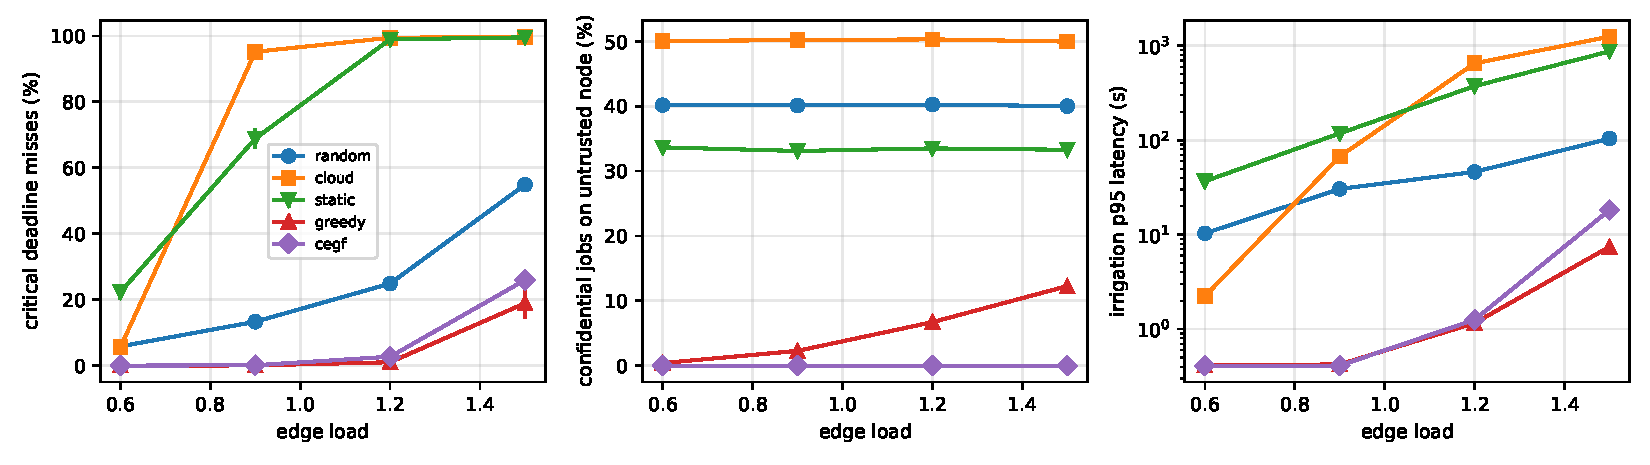
\includegraphics[width=\textwidth]{results/fig_e2.pdf}
\caption{E2: critical misses, confidential jobs on untrusted nodes, and irrigation p95 latency vs.\ edge load.}\label{fig:e2}
\end{figure}

\paragraph{E2b -- sensitivity to $\alpha$ and $\tau$ (load 1.2).}
\begin{table}[htbp]\scriptsize\centering
\caption{E2b -- sensitivity of CEGF to $\alpha$ and $\tau$ at load 1.2 (20 seeds).}\label{tab:e2-thr}
\begin{tabular}{lrrrr}
\toprule
$\alpha$ / $\tau$ & Critical misses (\%) & Disease-job misses (\%) & Fallback (\%) & Rejected (\%) \\
\midrule
0.0 / 0.5 & 0.5\,$\pm$\,0.3 & 0.0\,$\pm$\,0.0 & 0.0\,$\pm$\,0.0 & 0.0\,$\pm$\,0.0 \\
0.0 / 0.7 & 0.4\,$\pm$\,0.3 & 0.7\,$\pm$\,1.4 & 0.0\,$\pm$\,0.0 & 0.0\,$\pm$\,0.0 \\
0.0 / 0.9 & 9.6\,$\pm$\,2.5 & 46.5\,$\pm$\,15.6 & 0.0\,$\pm$\,0.0 & 0.0\,$\pm$\,0.0 \\
0.0 / 0.96 & 18.2\,$\pm$\,0.2 & 100.0\,$\pm$\,0.0 & 35.0\,$\pm$\,0.2 & 35.0\,$\pm$\,0.2 \\
0.25 / 0.5 & 0.5\,$\pm$\,0.3 & 0.0\,$\pm$\,0.0 & 0.2\,$\pm$\,0.2 & 0.0\,$\pm$\,0.0 \\
0.25 / 0.7 & 2.7\,$\pm$\,0.7 & 0.3\,$\pm$\,0.7 & 2.0\,$\pm$\,0.3 & 0.3\,$\pm$\,0.2 \\
0.25 / 0.9 & 11.7\,$\pm$\,1.2 & 8.5\,$\pm$\,6.3 & 7.7\,$\pm$\,0.4 & 4.9\,$\pm$\,0.5 \\
0.25 / 0.96 & 18.2\,$\pm$\,0.2 & 100.0\,$\pm$\,0.0 & 35.0\,$\pm$\,0.2 & 35.0\,$\pm$\,0.2 \\
0.5 / 0.5 & 0.7\,$\pm$\,0.4 & 0.0\,$\pm$\,0.0 & 0.4\,$\pm$\,0.2 & 0.0\,$\pm$\,0.0 \\
0.5 / 0.7 & 2.9\,$\pm$\,0.8 & 0.4\,$\pm$\,0.8 & 3.1\,$\pm$\,0.4 & 0.4\,$\pm$\,0.2 \\
0.5 / 0.9 & 12.5\,$\pm$\,1.1 & 8.4\,$\pm$\,6.3 & 8.5\,$\pm$\,0.4 & 5.4\,$\pm$\,0.5 \\
0.5 / 0.96 & 18.2\,$\pm$\,0.2 & 100.0\,$\pm$\,0.0 & 35.0\,$\pm$\,0.2 & 35.0\,$\pm$\,0.2 \\
0.75 / 0.5 & 1.6\,$\pm$\,0.7 & 0.0\,$\pm$\,0.0 & 1.2\,$\pm$\,0.4 & 0.0\,$\pm$\,0.0 \\
0.75 / 0.7 & 7.6\,$\pm$\,1.3 & 0.5\,$\pm$\,1.1 & 8.1\,$\pm$\,0.7 & 0.7\,$\pm$\,0.2 \\
0.75 / 0.9 & 23.3\,$\pm$\,1.5 & 11.5\,$\pm$\,7.9 & 15.3\,$\pm$\,1.0 & 6.7\,$\pm$\,0.4 \\
0.75 / 0.96 & 18.2\,$\pm$\,0.2 & 100.0\,$\pm$\,0.0 & 35.0\,$\pm$\,0.2 & 35.0\,$\pm$\,0.2 \\
\bottomrule
\end{tabular}
\end{table}
$\alpha=0$ disables the availability prohibition: at $\tau$=0.9 critical misses reach 9.6\,\%, and misses rise
with larger $\alpha$ too (7.6\,\% at $\alpha$=0.75, $\tau$=0.7) because fewer nodes qualify. $\tau$ drives the cost:
at $\tau$=0.9 only $e_{n1}$ and $c_{n1}$ qualify and 4.9\,\% of jobs are rejected. At $\tau$=0.96 \emph{no} node
qualifies, so every confidential job is rejected (35\,\%) and critical misses reach 18\,\%. This is the situation
the draft warns about (no node satisfies both thresholds); the fallback only mitigates it.

\subsection{E3: flexibility}
At $t$=900\,s of a 30-minute run we tighten the policy to $\alpha$=0.5, $\tau$=0.9. CEGF replaces the ODRL parameters
at run time and the next decision uses them; jobs already placed are untouched. The comparison is a
hard-coded policy that needs a 30\,s redeploy (an \emph{assumed} outage, during which no placement decision is made).
\begin{table}[htbp]\scriptsize\centering
\caption{E3 -- policy change at $t$=900\,s ($\alpha$: 0.25$\to$0.5, $\tau$: 0.7$\to$0.9). Violations audited against the policy in force at decision time.}\label{tab:e3}
\begin{tabular}{lrrrr}
\toprule
Setup & Crit.\ miss pre (\%) & Crit.\ miss post (\%) & Violations (\%) & Conf.\ viol.\ (\%) \\
\midrule
no change & 0.4\,$\pm$\,0.2 & 0.5\,$\pm$\,0.3 & 0.0\,$\pm$\,0.0 & 0.0\,$\pm$\,0.0 \\
CEGF (runtime swap) & 0.4\,$\pm$\,0.2 & 2.4\,$\pm$\,0.7 & 0.0\,$\pm$\,0.0 & 0.0\,$\pm$\,0.0 \\
hard-coded (30 s redeploy) & 0.4\,$\pm$\,0.2 & 7.7\,$\pm$\,0.8 & 0.0\,$\pm$\,0.0 & 0.0\,$\pm$\,0.0 \\
\bottomrule
\end{tabular}
\end{table}
After the change, CEGF has zero violations under the \emph{new} policy and keeps serving: critical misses rise from
0.4\,\% to 2.4\,\% (a stricter policy leaves fewer eligible nodes, as in E2b), versus 7.7\,\% for the redeploy
baseline. Evaluating the policy costs about 4--8\,$\mu$s per node check in this implementation.

\begin{figure}[htbp]\centering
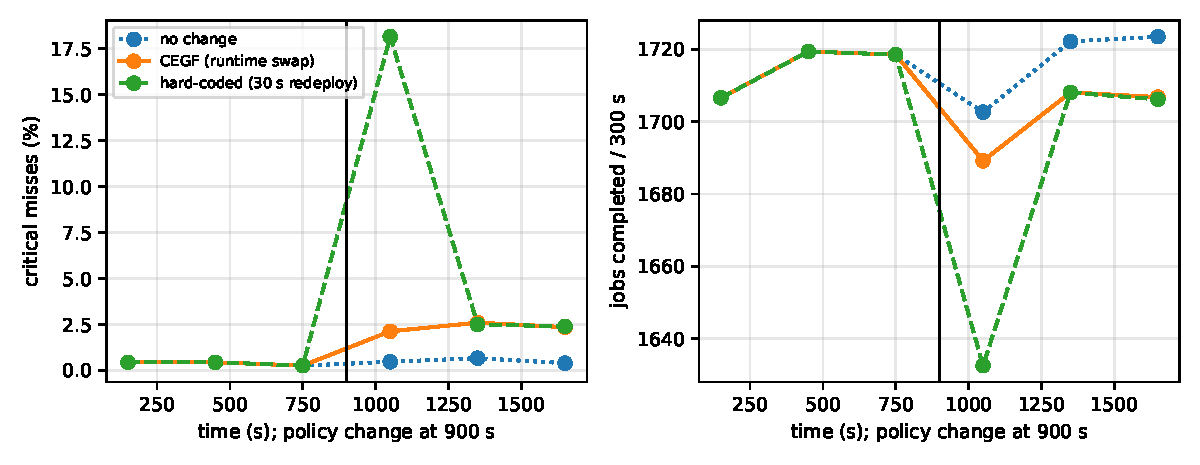
\includegraphics[width=.7\textwidth]{results/fig_e3.pdf}
\caption{E3: critical misses and completed jobs per 300\,s window around a policy change at 900\,s.}\label{fig:e3}
\end{figure}


\subsection{Replication on iFogSim2}\label{sec:ifogsim}
To check that the conclusions do not depend on our own simulator, we re-ran the same experiments on iFogSim2
(\texttt{src/org/fog/cegf/}): the gateways, the shared 2\,Mbit/s uplink, and the cloud are iFogSim2 entities, peer
offloading uses its cluster links, and the same ODRL JSON files are evaluated by a Java evaluator. Differences from
Section~\ref{sec:experiments}'s simulator: iFogSim2 shares a node's CPU among running tuples (processor sharing)
instead of FIFO slots; there is one cloud node (trust 0.95) and no edge failures; the data window is 1\,h. 20 seeds.

\paragraph{Data flow.} The results agree closely (Fig.~\ref{fig:sim-agree}). At nominal load, CEGF forwards 43.8\,\%
of the items, which cuts uplink traffic from 17.8\,MB/h (ungoverned) and 27.3\,MB/h (all-HTTPS) to 11.7\,MB/h, with no
useful reading lost in transit (ungoverned: 1.9\,\%). The timely-useful ratio is 98.8\,\% for CEGF, 98.0\,\% for
ungoverned, and 99.6\,\% for all-HTTPS. With 50\,\% more cameras both baselines collapse (8\,\% and 1.5\,\%), while CEGF
stays at 98.7\,\%. The $\theta$ curve is practically identical to the Python one ($\theta$=0.3: recall 98.8\,\%,
44\,\% forwarded; $\theta$=0.7: recall 58\,\%).

\paragraph{Job distribution.} CEGF again has zero policy violations at every load. At load 0.9 it has 0.01\,\% critical
misses, while greedy has 0.00\,\% but violates the policy for 3.0\,\% of jobs (6.4\,\% of confidential jobs on an
untrusted node). At load 1.2 CEGF misses 0.9\,\% of critical deadlines (greedy: 0.1\,\%, with 7.1\,\% violations and
9.5\,\% confidential jobs on untrusted nodes); at load 1.5 the price of compliance is larger (16.3\,\% vs.\ 2.6\,\%
critical misses, 17\,\% of jobs using the fallback; greedy violates the policy for 19.9\,\%). Random (74\,\% misses at
1.5), static, and cloud-only are far worse. The ranking is the same as in the first simulator, but iFogSim2's
processor sharing makes the strong strategies look better (CEGF 0.9\,\% vs.\ 2.7\,\% critical misses at load 1.2) and
random worse (56\,\% vs.\ 25\,\%).

\paragraph{Thresholds and flexibility.} The $\alpha$/$\tau$ grid reproduces the pattern: critical misses grow with
$\tau$ (8.0\,\% at $\tau$=0.9, $\alpha$=0.25), and at $\tau$=0.96 no node qualifies, so all confidential jobs fail
(34.9\,\% of jobs are rejected, 18.1\,\% critical misses). When the policy is tightened at 900\,s, the runtime swap keeps
critical misses at 1.1\,\% (0.1\,\% before), against 6.7\,\% for the assumed 30\,s redeploy; no violations occur in either
case.

\begin{figure}[htbp]\centering
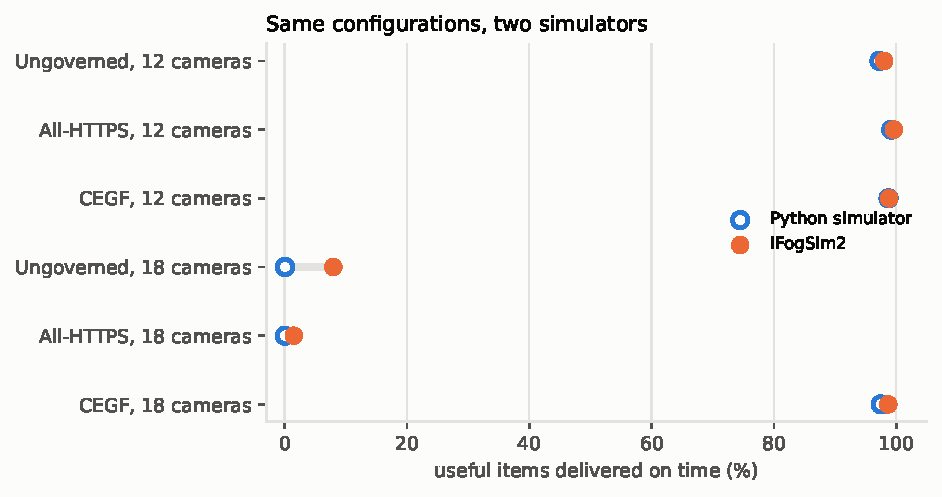
\includegraphics[width=.6	extwidth]{../ifogsim/results/visuals/fig5_simulator_agreement.pdf}
\caption{Timely-useful ratio for the same configurations in both simulators.}\label{fig:sim-agree}
\end{figure}

\subsection{Threats to validity}
(i) The simulator, workloads, trust and availability values, and the 30\,s redeploy outage are assumptions; the
absolute numbers are illustrative and the comparisons are what matter. (ii) Readings and frames share one FIFO queue
at each gateway, and the uplink is a fluid model; this makes the overload collapse in E1a sharper than in a system
with separate queues. (iii) \textsf{UG}, \textsf{cloud-only}, and \textsf{static} are deliberately weak reference
points; \textsf{greedy} and \textsf{SS} are the informative baselines. (iv) $H(d)$ is a synthetic proxy of
usefulness, and $\theta$, $\alpha$, $\tau$ were not tuned on real farm data. (v) $\mathcal{DF}_5$ is not evaluated and
$\mathcal{DF}_4$ has no policies yet. (vi) The iFogSim2 port uses one cloud node, no failures, and none of iFogSim2's mobility or microservice features.
